\documentclass[1p]{elsarticle_modified}
%\bibliographystyle{elsarticle-num}

%\usepackage[colorlinks]{hyperref}
%\usepackage{abbrmath_seonhwa} %\Abb, \Ascr, \Acal ,\Abf, \Afrak
\usepackage{amsfonts}
\usepackage{amssymb}
\usepackage{amsmath}
\usepackage{amsthm}
\usepackage{scalefnt}
\usepackage{amsbsy}
\usepackage{kotex}
\usepackage{caption}
\usepackage{subfig}
\usepackage{color}
\usepackage{graphicx}
\usepackage{xcolor} %% white, black, red, green, blue, cyan, magenta, yellow
\usepackage{float}
\usepackage{setspace}
\usepackage{hyperref}

\usepackage{tikz}
\usetikzlibrary{arrows}

\usepackage{multirow}
\usepackage{array} % fixed length table
\usepackage{hhline}

%%%%%%%%%%%%%%%%%%%%%
\makeatletter
\renewcommand*\env@matrix[1][\arraystretch]{%
	\edef\arraystretch{#1}%
	\hskip -\arraycolsep
	\let\@ifnextchar\new@ifnextchar
	\array{*\c@MaxMatrixCols c}}
\makeatother %https://tex.stackexchange.com/questions/14071/how-can-i-increase-the-line-spacing-in-a-matrix
%%%%%%%%%%%%%%%

\usepackage[normalem]{ulem}

\newcommand{\msout}[1]{\ifmmode\text{\sout{\ensuremath{#1}}}\else\sout{#1}\fi}
%SOURCE: \msout is \stkout macro in https://tex.stackexchange.com/questions/20609/strikeout-in-math-mode

\newcommand{\cancel}[1]{
	\ifmmode
	{\color{red}\msout{#1}}
	\else
	{\color{red}\sout{#1}}
	\fi
}

\newcommand{\add}[1]{
	{\color{blue}\uwave{#1}}
}

\newcommand{\replace}[2]{
	\ifmmode
	{\color{red}\msout{#1}}{\color{blue}\uwave{#2}}
	\else
	{\color{red}\sout{#1}}{\color{blue}\uwave{#2}}
	\fi
}

\newcommand{\Sol}{\mathcal{S}} %segment
\newcommand{\D}{D} %diagram
\newcommand{\A}{\mathcal{A}} %arc


%%%%%%%%%%%%%%%%%%%%%%%%%%%%%5 test

\def\sl{\operatorname{\textup{SL}}(2,\Cbb)}
\def\psl{\operatorname{\textup{PSL}}(2,\Cbb)}
\def\quan{\mkern 1mu \triangleright \mkern 1mu}

\theoremstyle{definition}
\newtheorem{thm}{Theorem}[section]
\newtheorem{prop}[thm]{Proposition}
\newtheorem{lem}[thm]{Lemma}
\newtheorem{ques}[thm]{Question}
\newtheorem{cor}[thm]{Corollary}
\newtheorem{defn}[thm]{Definition}
\newtheorem{exam}[thm]{Example}
\newtheorem{rmk}[thm]{Remark}
\newtheorem{alg}[thm]{Algorithm}

\newcommand{\I}{\sqrt{-1}}
\begin{document}

%\begin{frontmatter}
%
%\title{Boundary parabolic representations of knots up to 8 crossings}
%
%%% Group authors per affiliation:
%\author{Yunhi Cho} 
%\address{Department of Mathematics, University of Seoul, Seoul, Korea}
%\ead{yhcho@uos.ac.kr}
%
%
%\author{Seonhwa Kim} %\fnref{s_kim}}
%\address{Center for Geometry and Physics, Institute for Basic Science, Pohang, 37673, Korea}
%\ead{ryeona17@ibs.re.kr}
%
%\author{Hyuk Kim}
%\address{Department of Mathematical Sciences, Seoul National University, Seoul 08826, Korea}
%\ead{hyukkim@snu.ac.kr}
%
%\author{Seokbeom Yoon}
%\address{Department of Mathematical Sciences, Seoul National University, Seoul, 08826,  Korea}
%\ead{sbyoon15@snu.ac.kr}
%
%\begin{abstract}
%We find all boundary parabolic representation of knots up to 8 crossings.
%
%\end{abstract}
%\begin{keyword}
%    \MSC[2010] 57M25 
%\end{keyword}
%
%\end{frontmatter}

%\linenumbers
%\tableofcontents
%
\newcommand\colored[1]{\textcolor{white}{\rule[-0.35ex]{0.8em}{1.4ex}}\kern-0.8em\color{red} #1}%
%\newcommand\colored[1]{\textcolor{white}{ #1}\kern-2.17ex	\textcolor{white}{ #1}\kern-1.81ex	\textcolor{white}{ #1}\kern-2.15ex\color{red}#1	}

{\Large $\underline{11a_{187}~(K11a_{187})}$}

\setlength{\tabcolsep}{10pt}
\renewcommand{\arraystretch}{1.6}
\vspace{1cm}\begin{tabular}{m{100pt}>{\centering\arraybackslash}m{274pt}}
\multirow{5}{120pt}{
	\centering
	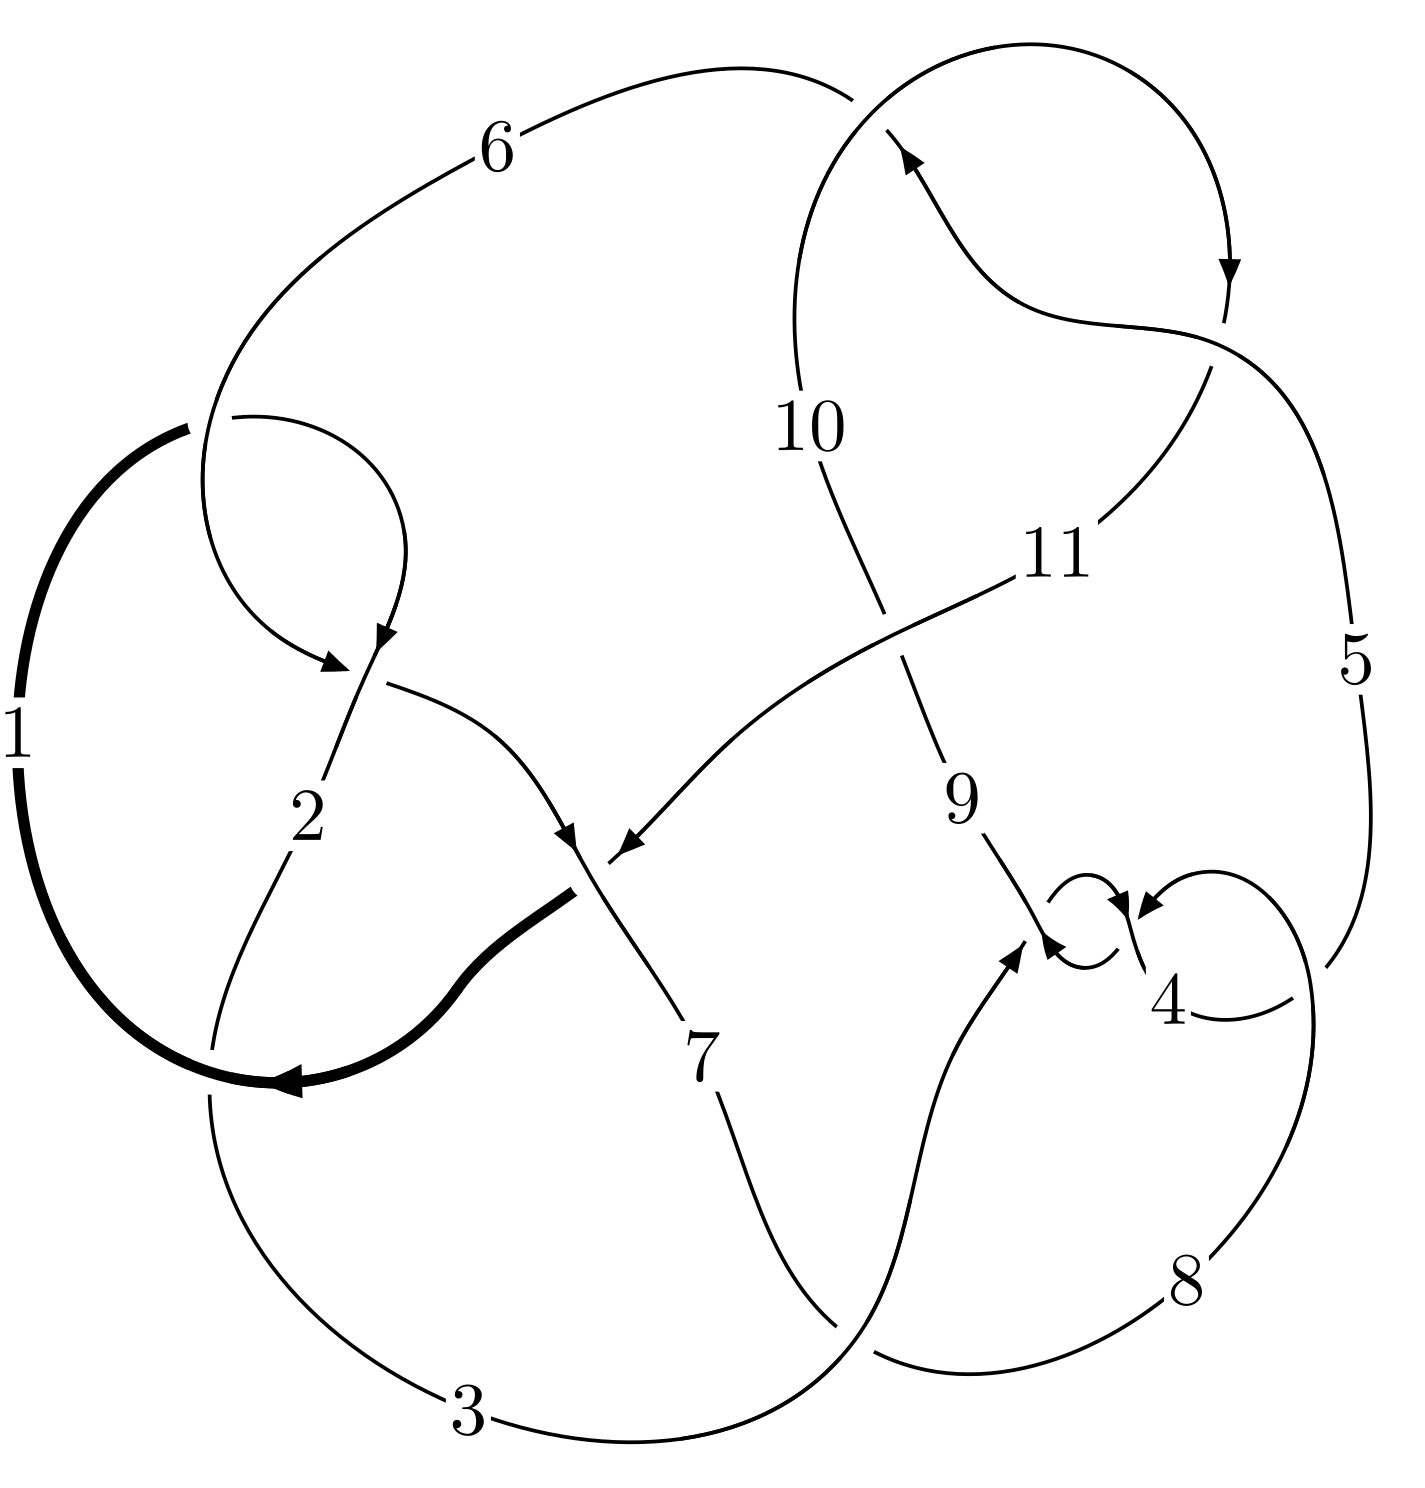
\includegraphics[width=112pt]{../../../GIT/diagram.site/Diagrams/png/436_11a_187.png}\\
\ \ \ A knot diagram\footnotemark}&
\allowdisplaybreaks
\textbf{Linearized knot diagam} \\
\cline{2-2}
 &
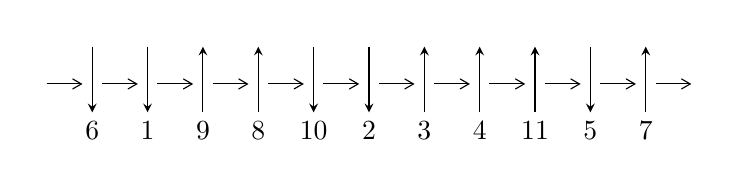
\begin{tikzpicture}[x=20pt, y=17pt]
	% nodes
	\node (C0) at (0, 0) {};
	\node (C1) at (1, 0) {};
	\node (C1U) at (1, +1) {};
	\node (C1D) at (1, -1) {6};

	\node (C2) at (2, 0) {};
	\node (C2U) at (2, +1) {};
	\node (C2D) at (2, -1) {1};

	\node (C3) at (3, 0) {};
	\node (C3U) at (3, +1) {};
	\node (C3D) at (3, -1) {9};

	\node (C4) at (4, 0) {};
	\node (C4U) at (4, +1) {};
	\node (C4D) at (4, -1) {8};

	\node (C5) at (5, 0) {};
	\node (C5U) at (5, +1) {};
	\node (C5D) at (5, -1) {10};

	\node (C6) at (6, 0) {};
	\node (C6U) at (6, +1) {};
	\node (C6D) at (6, -1) {2};

	\node (C7) at (7, 0) {};
	\node (C7U) at (7, +1) {};
	\node (C7D) at (7, -1) {3};

	\node (C8) at (8, 0) {};
	\node (C8U) at (8, +1) {};
	\node (C8D) at (8, -1) {4};

	\node (C9) at (9, 0) {};
	\node (C9U) at (9, +1) {};
	\node (C9D) at (9, -1) {11};

	\node (C10) at (10, 0) {};
	\node (C10U) at (10, +1) {};
	\node (C10D) at (10, -1) {5};

	\node (C11) at (11, 0) {};
	\node (C11U) at (11, +1) {};
	\node (C11D) at (11, -1) {7};
	\node (C12) at (12, 0) {};

	% arrows
	\draw[->,>={angle 60}]
	(C0) edge (C1) (C1) edge (C2) (C2) edge (C3) (C3) edge (C4) (C4) edge (C5) (C5) edge (C6) (C6) edge (C7) (C7) edge (C8) (C8) edge (C9) (C9) edge (C10) (C10) edge (C11) (C11) edge (C12) ;	\draw[->,>=stealth]
	(C1U) edge (C1D) (C2U) edge (C2D) (C3D) edge (C3U) (C4D) edge (C4U) (C5U) edge (C5D) (C6U) edge (C6D) (C7D) edge (C7U) (C8D) edge (C8U) (C9D) edge (C9U) (C10U) edge (C10D) (C11D) edge (C11U) ;
	\end{tikzpicture} \\
\hhline{~~} \\& 
\textbf{Solving Sequence} \\ \cline{2-2} 
 &
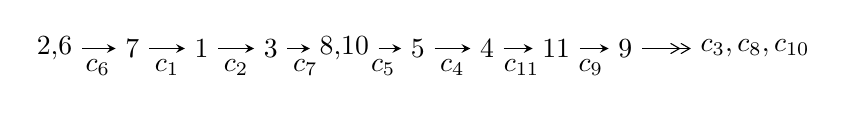
\begin{tikzpicture}[x=25pt, y=7pt]
	% node
	\node (A0) at (-1/8, 0) {2,6};
	\node (A1) at (1, 0) {7};
	\node (A2) at (2, 0) {1};
	\node (A3) at (3, 0) {3};
	\node (A4) at (65/16, 0) {8,10};
	\node (A5) at (41/8, 0) {5};
	\node (A6) at (49/8, 0) {4};
	\node (A7) at (57/8, 0) {11};
	\node (A8) at (65/8, 0) {9};
	\node (C1) at (1/2, -1) {$c_{6}$};
	\node (C2) at (3/2, -1) {$c_{1}$};
	\node (C3) at (5/2, -1) {$c_{2}$};
	\node (C4) at (7/2, -1) {$c_{7}$};
	\node (C5) at (37/8, -1) {$c_{5}$};
	\node (C6) at (45/8, -1) {$c_{4}$};
	\node (C7) at (53/8, -1) {$c_{11}$};
	\node (C8) at (61/8, -1) {$c_{9}$};
	\node (A9) at (10, 0) {$c_{3},c_{8},c_{10}$};

	% edge
	\draw[->,>=stealth]	
	(A0) edge (A1) (A1) edge (A2) (A2) edge (A3) (A3) edge (A4) (A4) edge (A5) (A5) edge (A6) (A6) edge (A7) (A7) edge (A8) ;
	\draw[->>,>={angle 60}]	
	(A8) edge (A9);
\end{tikzpicture} \\ 

\end{tabular} \\

\footnotetext{
The image of knot diagram is generated by the software ``\textbf{Draw programme}" developed by Andrew Bartholomew(\url{http://www.layer8.co.uk/maths/draw/index.htm\#Running-draw}), where we modified some parts for our purpose(\url{https://github.com/CATsTAILs/LinksPainter}).
}\phantom \\ \newline 
\centering \textbf{Ideals for irreducible components\footnotemark of $X_{\text{par}}$} 
 
\begin{align*}
I^u_{1}&=\langle 
2 u^{43}+2 u^{42}+\cdots+4 b+2,\;2 u^{43}+u^{42}+\cdots+4 a+4,\;u^{44}+2 u^{43}+\cdots+3 u+2\rangle \\
I^u_{2}&=\langle 
-42 u^5 a^2+6 u^5 a+\cdots-33 a-16,\\
\phantom{I^u_{2}}&\phantom{= \langle  }2 u^4 a^2+u^5 a-2 u^3 a^2+2 u^4 a+u^5-2 a^2 u^2- u^4+a^3+2 a^2 u-3 u^2 a+u^3+2 a u+2 u^2+a-2 u+1,\\
\phantom{I^u_{2}}&\phantom{= \langle  }u^6- u^5- u^4+2 u^3- u+1\rangle \\
I^u_{3}&=\langle 
u^3+b,\;- u^3- u^2+a+u+1,\;u^4- u^2+1\rangle \\
\\
\end{align*}
\raggedright * 3 irreducible components of $\dim_{\mathbb{C}}=0$, with total 66 representations.\\
\footnotetext{All coefficients of polynomials are rational numbers. But the coefficients are sometimes approximated in decimal forms when there is not enough margin.}
\newpage
\renewcommand{\arraystretch}{1}
\centering \section*{I. $I^u_{1}= \langle 2 u^{43}+2 u^{42}+\cdots+4 b+2,\;2 u^{43}+u^{42}+\cdots+4 a+4,\;u^{44}+2 u^{43}+\cdots+3 u+2 \rangle$}
\flushleft \textbf{(i) Arc colorings}\\
\begin{tabular}{m{7pt} m{180pt} m{7pt} m{180pt} }
\flushright $a_{2}=$&$\begin{pmatrix}0\\u\end{pmatrix}$ \\
\flushright $a_{6}=$&$\begin{pmatrix}1\\0\end{pmatrix}$ \\
\flushright $a_{7}=$&$\begin{pmatrix}1\\u^2\end{pmatrix}$ \\
\flushright $a_{1}=$&$\begin{pmatrix}u\\u\end{pmatrix}$ \\
\flushright $a_{3}=$&$\begin{pmatrix}- u^3\\- u^3+u\end{pmatrix}$ \\
\flushright $a_{8}=$&$\begin{pmatrix}u^8- u^6+u^4+1\\u^8-2 u^6+2 u^4\end{pmatrix}$ \\
\flushright $a_{10}=$&$\begin{pmatrix}-\frac{1}{2} u^{43}-\frac{1}{4} u^{42}+\cdots-\frac{1}{4} u-1\\-\frac{1}{2} u^{43}-\frac{1}{2} u^{42}+\cdots+\frac{1}{4} u-\frac{1}{2}\end{pmatrix}$ \\
\flushright $a_{5}=$&$\begin{pmatrix}\frac{1}{2} u^{43}-5 u^{41}+\cdots+\frac{9}{4} u+1\\-\frac{1}{4} u^{39}+\frac{9}{4} u^{37}+\cdots+\frac{1}{2} u+1\end{pmatrix}$ \\
\flushright $a_{4}=$&$\begin{pmatrix}-\frac{1}{4} u^{34}+\frac{7}{4} u^{32}+\cdots+\frac{1}{2} u+\frac{1}{2}\\-\frac{1}{4} u^{36}+2 u^{34}+\cdots-\frac{3}{4} u^2+u\end{pmatrix}$ \\
\flushright $a_{11}=$&$\begin{pmatrix}u^3\\u^5- u^3+u\end{pmatrix}$ \\
\flushright $a_{9}=$&$\begin{pmatrix}-\frac{1}{2} u^{43}+5 u^{41}+\cdots-\frac{1}{4} u-1\\- u^{43}- u^{42}+\cdots-\frac{3}{2} u-1\end{pmatrix}$\\ \flushright $a_{9}=$&$\begin{pmatrix}-\frac{1}{2} u^{43}+5 u^{41}+\cdots-\frac{1}{4} u-1\\- u^{43}- u^{42}+\cdots-\frac{3}{2} u-1\end{pmatrix}$\\&\end{tabular}
\flushleft \textbf{(ii) Obstruction class $= -1$}\\~\\
\flushleft \textbf{(iii) Cusp Shapes $= -2 u^{43}+20 u^{41}+4 u^{40}-104 u^{39}-36 u^{38}+356 u^{37}+168 u^{36}-886 u^{35}-516 u^{34}+1682 u^{33}+1152 u^{32}-2512 u^{31}-1966 u^{30}+3018 u^{29}+2658 u^{28}-2988 u^{27}-2940 u^{26}+2506 u^{25}+2762 u^{24}-1828 u^{23}-2288 u^{22}+1160 u^{21}+1706 u^{20}-614 u^{19}-1138 u^{18}+234 u^{17}+680 u^{16}-8 u^{15}-356 u^{14}-126 u^{13}+132 u^{12}+148 u^{11}+30 u^{10}-90 u^9-66 u^8+36 u^6+8 u^5+12 u^4-4 u^3-4 u^2-12 u+2$}\\~\\
\newpage\renewcommand{\arraystretch}{1}
\flushleft \textbf{(iv) u-Polynomials at the component}\newline \\
\begin{tabular}{m{50pt}|m{274pt}}
Crossings & \hspace{64pt}u-Polynomials at each crossing \\
\hline $$\begin{aligned}c_{1},c_{6}\end{aligned}$$&$\begin{aligned}
&u^{44}+2 u^{43}+\cdots+3 u+2
\end{aligned}$\\
\hline $$\begin{aligned}c_{2}\end{aligned}$$&$\begin{aligned}
&u^{44}+20 u^{43}+\cdots-19 u+4
\end{aligned}$\\
\hline $$\begin{aligned}c_{3},c_{4},c_{8}\end{aligned}$$&$\begin{aligned}
&u^{44}- u^{43}+\cdots-16 u+1
\end{aligned}$\\
\hline $$\begin{aligned}c_{5},c_{10}\end{aligned}$$&$\begin{aligned}
&u^{44}- u^{43}+\cdots-2 u+1
\end{aligned}$\\
\hline $$\begin{aligned}c_{7}\end{aligned}$$&$\begin{aligned}
&u^{44}-2 u^{43}+\cdots-496 u+32
\end{aligned}$\\
\hline $$\begin{aligned}c_{9}\end{aligned}$$&$\begin{aligned}
&u^{44}-21 u^{43}+\cdots-6 u+1
\end{aligned}$\\
\hline $$\begin{aligned}c_{11}\end{aligned}$$&$\begin{aligned}
&u^{44}+6 u^{43}+\cdots+352 u+128
\end{aligned}$\\
\hline
\end{tabular}\\~\\
\newpage\renewcommand{\arraystretch}{1}
\flushleft \textbf{(v) Riley Polynomials at the component}\newline \\
\begin{tabular}{m{50pt}|m{274pt}}
Crossings & \hspace{64pt}Riley Polynomials at each crossing \\
\hline $$\begin{aligned}c_{1},c_{6}\end{aligned}$$&$\begin{aligned}
&y^{44}-20 y^{43}+\cdots+19 y+4
\end{aligned}$\\
\hline $$\begin{aligned}c_{2}\end{aligned}$$&$\begin{aligned}
&y^{44}+8 y^{43}+\cdots-417 y+16
\end{aligned}$\\
\hline $$\begin{aligned}c_{3},c_{4},c_{8}\end{aligned}$$&$\begin{aligned}
&y^{44}+41 y^{43}+\cdots-90 y+1
\end{aligned}$\\
\hline $$\begin{aligned}c_{5},c_{10}\end{aligned}$$&$\begin{aligned}
&y^{44}+21 y^{43}+\cdots+6 y+1
\end{aligned}$\\
\hline $$\begin{aligned}c_{7}\end{aligned}$$&$\begin{aligned}
&y^{44}-18 y^{43}+\cdots-81664 y+1024
\end{aligned}$\\
\hline $$\begin{aligned}c_{9}\end{aligned}$$&$\begin{aligned}
&y^{44}+9 y^{43}+\cdots+26 y+1
\end{aligned}$\\
\hline $$\begin{aligned}c_{11}\end{aligned}$$&$\begin{aligned}
&y^{44}+4 y^{43}+\cdots+400384 y+16384
\end{aligned}$\\
\hline
\end{tabular}\\~\\
\newpage\flushleft \textbf{(vi) Complex Volumes and Cusp Shapes}
$$\begin{array}{c|c|c}  
\text{Solutions to }I^u_{1}& \I (\text{vol} + \sqrt{-1}CS) & \text{Cusp shape}\\
 \hline 
\begin{aligned}
u &= \phantom{-}0.614083 + 0.757021 I \\
a &= -0.632443 + 1.216370 I \\
b &= -0.484382 - 1.114490 I\end{aligned}
 & \phantom{-}1.31355 - 6.59166 I & \phantom{-}2.43428 + 6.77222 I \\ \hline\begin{aligned}
u &= \phantom{-}0.614083 - 0.757021 I \\
a &= -0.632443 - 1.216370 I \\
b &= -0.484382 + 1.114490 I\end{aligned}
 & \phantom{-}1.31355 + 6.59166 I & \phantom{-}2.43428 - 6.77222 I \\ \hline\begin{aligned}
u &= \phantom{-}0.821139 + 0.488156 I \\
a &= -0.927633 + 0.608891 I \\
b &= -0.072544 - 0.992801 I\end{aligned}
 & \phantom{-}1.71974 - 2.04449 I & \phantom{-}8.09534 + 3.92627 I \\ \hline\begin{aligned}
u &= \phantom{-}0.821139 - 0.488156 I \\
a &= -0.927633 - 0.608891 I \\
b &= -0.072544 + 0.992801 I\end{aligned}
 & \phantom{-}1.71974 + 2.04449 I & \phantom{-}8.09534 - 3.92627 I \\ \hline\begin{aligned}
u &= -0.862505 + 0.618420 I \\
a &= \phantom{-}0.449298 + 0.919851 I \\
b &= \phantom{-}0.296344 - 0.458666 I\end{aligned}
 & -1.78260 + 2.32403 I & -3.34006 - 4.18594 I \\ \hline\begin{aligned}
u &= -0.862505 - 0.618420 I \\
a &= \phantom{-}0.449298 - 0.919851 I \\
b &= \phantom{-}0.296344 + 0.458666 I\end{aligned}
 & -1.78260 - 2.32403 I & -3.34006 + 4.18594 I \\ \hline\begin{aligned}
u &= \phantom{-}1.073220 + 0.159361 I \\
a &= -1.46758 + 0.81560 I \\
b &= -0.486107 + 1.058250 I\end{aligned}
 & -0.00015 + 3.23140 I & -0.12341 - 4.01153 I \\ \hline\begin{aligned}
u &= \phantom{-}1.073220 - 0.159361 I \\
a &= -1.46758 - 0.81560 I \\
b &= -0.486107 - 1.058250 I\end{aligned}
 & -0.00015 - 3.23140 I & -0.12341 + 4.01153 I \\ \hline\begin{aligned}
u &= -0.650664 + 0.627229 I \\
a &= -0.005189 + 0.303137 I \\
b &= -0.553759 - 0.162746 I\end{aligned}
 & -1.24285 + 2.41947 I & -1.11371 - 3.27345 I \\ \hline\begin{aligned}
u &= -0.650664 - 0.627229 I \\
a &= -0.005189 - 0.303137 I \\
b &= -0.553759 + 0.162746 I\end{aligned}
 & -1.24285 - 2.41947 I & -1.11371 + 3.27345 I\\
 \hline 
 \end{array}$$\newpage$$\begin{array}{c|c|c}  
\text{Solutions to }I^u_{1}& \I (\text{vol} + \sqrt{-1}CS) & \text{Cusp shape}\\
 \hline 
\begin{aligned}
u &= \phantom{-}0.383154 + 0.817621 I \\
a &= -0.699793 - 1.003430 I \\
b &= -0.559403 + 1.175300 I\end{aligned}
 & \phantom{-}0.02553 + 9.64814 I & \phantom{-}1.87633 - 5.89081 I \\ \hline\begin{aligned}
u &= \phantom{-}0.383154 - 0.817621 I \\
a &= -0.699793 + 1.003430 I \\
b &= -0.559403 - 1.175300 I\end{aligned}
 & \phantom{-}0.02553 - 9.64814 I & \phantom{-}1.87633 + 5.89081 I \\ \hline\begin{aligned}
u &= -0.541524 + 0.710426 I \\
a &= \phantom{-}0.69602 + 1.31058 I \\
b &= \phantom{-}0.390858 - 1.163740 I\end{aligned}
 & \phantom{-}5.49978 + 2.81685 I & \phantom{-}7.91209 - 3.62313 I \\ \hline\begin{aligned}
u &= -0.541524 - 0.710426 I \\
a &= \phantom{-}0.69602 - 1.31058 I \\
b &= \phantom{-}0.390858 + 1.163740 I\end{aligned}
 & \phantom{-}5.49978 - 2.81685 I & \phantom{-}7.91209 + 3.62313 I \\ \hline\begin{aligned}
u &= -1.012810 + 0.465132 I \\
a &= \phantom{-}0.56553 + 1.48232 I \\
b &= \phantom{-}0.441089 + 0.401407 I\end{aligned}
 & -2.03263 + 1.73845 I & -4.12033 - 0.48900 I \\ \hline\begin{aligned}
u &= -1.012810 - 0.465132 I \\
a &= \phantom{-}0.56553 - 1.48232 I \\
b &= \phantom{-}0.441089 - 0.401407 I\end{aligned}
 & -2.03263 - 1.73845 I & -4.12033 + 0.48900 I \\ \hline\begin{aligned}
u &= -0.406877 + 0.760900 I \\
a &= \phantom{-}0.879442 - 1.067170 I \\
b &= \phantom{-}0.490957 + 1.153170 I\end{aligned}
 & \phantom{-}4.79783 - 5.37629 I & \phantom{-}6.38044 + 4.26424 I \\ \hline\begin{aligned}
u &= -0.406877 - 0.760900 I \\
a &= \phantom{-}0.879442 + 1.067170 I \\
b &= \phantom{-}0.490957 - 1.153170 I\end{aligned}
 & \phantom{-}4.79783 + 5.37629 I & \phantom{-}6.38044 - 4.26424 I \\ \hline\begin{aligned}
u &= \phantom{-}1.059790 + 0.421005 I \\
a &= \phantom{-}2.19306 + 0.61348 I \\
b &= \phantom{-}0.508638 + 0.730201 I\end{aligned}
 & -2.20066 - 4.83120 I & -3.00848 + 8.38874 I \\ \hline\begin{aligned}
u &= \phantom{-}1.059790 - 0.421005 I \\
a &= \phantom{-}2.19306 - 0.61348 I \\
b &= \phantom{-}0.508638 - 0.730201 I\end{aligned}
 & -2.20066 + 4.83120 I & -3.00848 - 8.38874 I\\
 \hline 
 \end{array}$$\newpage$$\begin{array}{c|c|c}  
\text{Solutions to }I^u_{1}& \I (\text{vol} + \sqrt{-1}CS) & \text{Cusp shape}\\
 \hline 
\begin{aligned}
u &= \phantom{-}1.136200 + 0.221185 I \\
a &= \phantom{-}1.46732 + 0.20761 I \\
b &= \phantom{-}0.820180 + 0.375098 I\end{aligned}
 & -7.36306 + 1.79166 I & -7.40265 - 0.27193 I \\ \hline\begin{aligned}
u &= \phantom{-}1.136200 - 0.221185 I \\
a &= \phantom{-}1.46732 - 0.20761 I \\
b &= \phantom{-}0.820180 - 0.375098 I\end{aligned}
 & -7.36306 - 1.79166 I & -7.40265 + 0.27193 I \\ \hline\begin{aligned}
u &= -0.340701 + 0.765223 I \\
a &= -0.166604 - 0.002494 I \\
b &= -0.831807 + 0.245624 I\end{aligned}
 & -2.73686 - 4.51181 I & -1.28953 + 2.54030 I \\ \hline\begin{aligned}
u &= -0.340701 - 0.765223 I \\
a &= -0.166604 + 0.002494 I \\
b &= -0.831807 - 0.245624 I\end{aligned}
 & -2.73686 + 4.51181 I & -1.28953 - 2.54030 I \\ \hline\begin{aligned}
u &= -1.163100 + 0.154076 I \\
a &= \phantom{-}1.25749 + 0.76708 I \\
b &= \phantom{-}0.592275 + 1.120500 I\end{aligned}
 & -5.13953 - 7.03997 I & -4.35205 + 4.78449 I \\ \hline\begin{aligned}
u &= -1.163100 - 0.154076 I \\
a &= \phantom{-}1.25749 - 0.76708 I \\
b &= \phantom{-}0.592275 - 1.120500 I\end{aligned}
 & -5.13953 + 7.03997 I & -4.35205 - 4.78449 I \\ \hline\begin{aligned}
u &= -1.023700 + 0.599662 I \\
a &= \phantom{-}0.681062 + 0.160774 I \\
b &= -0.337241 - 1.172950 I\end{aligned}
 & \phantom{-}4.07169 + 2.20922 I & \phantom{-}5.83455 - 2.04205 I \\ \hline\begin{aligned}
u &= -1.023700 - 0.599662 I \\
a &= \phantom{-}0.681062 - 0.160774 I \\
b &= -0.337241 + 1.172950 I\end{aligned}
 & \phantom{-}4.07169 - 2.20922 I & \phantom{-}5.83455 + 2.04205 I \\ \hline\begin{aligned}
u &= \phantom{-}0.989262 + 0.656622 I \\
a &= -0.585610 + 0.177116 I \\
b &= \phantom{-}0.449630 - 1.070930 I\end{aligned}
 & \phantom{-}0.200378 + 1.249410 I & \phantom{-}0.49362 - 2.01846 I \\ \hline\begin{aligned}
u &= \phantom{-}0.989262 - 0.656622 I \\
a &= -0.585610 - 0.177116 I \\
b &= \phantom{-}0.449630 + 1.070930 I\end{aligned}
 & \phantom{-}0.200378 - 1.249410 I & \phantom{-}0.49362 + 2.01846 I\\
 \hline 
 \end{array}$$\newpage$$\begin{array}{c|c|c}  
\text{Solutions to }I^u_{1}& \I (\text{vol} + \sqrt{-1}CS) & \text{Cusp shape}\\
 \hline 
\begin{aligned}
u &= \phantom{-}1.154760 + 0.388979 I \\
a &= -0.93774 + 1.14513 I \\
b &= -0.753378 + 0.721249 I\end{aligned}
 & -9.26869 - 1.33308 I & -7.30769 + 0.69505 I \\ \hline\begin{aligned}
u &= \phantom{-}1.154760 - 0.388979 I \\
a &= -0.93774 - 1.14513 I \\
b &= -0.753378 - 0.721249 I\end{aligned}
 & -9.26869 + 1.33308 I & -7.30769 - 0.69505 I \\ \hline\begin{aligned}
u &= -1.155640 + 0.451289 I \\
a &= -2.06743 + 0.02294 I \\
b &= -0.716747 + 0.865040 I\end{aligned}
 & -8.84980 + 6.81745 I & -6.19135 - 6.52038 I \\ \hline\begin{aligned}
u &= -1.155640 - 0.451289 I \\
a &= -2.06743 - 0.02294 I \\
b &= -0.716747 - 0.865040 I\end{aligned}
 & -8.84980 - 6.81745 I & -6.19135 + 6.52038 I \\ \hline\begin{aligned}
u &= -1.101670 + 0.589261 I \\
a &= -2.50240 - 0.70880 I \\
b &= -0.527845 + 1.156650 I\end{aligned}
 & \phantom{-}2.74383 + 10.48610 I & \phantom{-}3.00784 - 8.49174 I \\ \hline\begin{aligned}
u &= -1.101670 - 0.589261 I \\
a &= -2.50240 + 0.70880 I \\
b &= -0.527845 - 1.156650 I\end{aligned}
 & \phantom{-}2.74383 - 10.48610 I & \phantom{-}3.00784 + 8.49174 I \\ \hline\begin{aligned}
u &= -1.123580 + 0.572511 I \\
a &= \phantom{-}0.627078 + 1.120360 I \\
b &= \phantom{-}0.896517 + 0.252922 I\end{aligned}
 & -5.03545 + 9.55347 I & -4.20919 - 6.36695 I \\ \hline\begin{aligned}
u &= -1.123580 - 0.572511 I \\
a &= \phantom{-}0.627078 - 1.120360 I \\
b &= \phantom{-}0.896517 - 0.252922 I\end{aligned}
 & -5.03545 - 9.55347 I & -4.20919 + 6.36695 I \\ \hline\begin{aligned}
u &= -0.068807 + 0.735625 I \\
a &= \phantom{-}0.599542 - 0.271859 I \\
b &= \phantom{-}0.657434 + 0.786735 I\end{aligned}
 & -5.68233 - 2.52073 I & -2.77619 + 3.16598 I \\ \hline\begin{aligned}
u &= -0.068807 - 0.735625 I \\
a &= \phantom{-}0.599542 + 0.271859 I \\
b &= \phantom{-}0.657434 - 0.786735 I\end{aligned}
 & -5.68233 + 2.52073 I & -2.77619 - 3.16598 I\\
 \hline 
 \end{array}$$\newpage$$\begin{array}{c|c|c}  
\text{Solutions to }I^u_{1}& \I (\text{vol} + \sqrt{-1}CS) & \text{Cusp shape}\\
 \hline 
\begin{aligned}
u &= \phantom{-}1.127870 + 0.601926 I \\
a &= \phantom{-}2.30965 - 0.72062 I \\
b &= \phantom{-}0.581039 + 1.195430 I\end{aligned}
 & -2.1965 - 14.9450 I & \phantom{-0.000000 -}0. + 9.66907 I \\ \hline\begin{aligned}
u &= \phantom{-}1.127870 - 0.601926 I \\
a &= \phantom{-}2.30965 + 0.72062 I \\
b &= \phantom{-}0.581039 - 1.195430 I\end{aligned}
 & -2.1965 + 14.9450 I & \phantom{-0.000000 } 0. - 9.66907 I \\ \hline\begin{aligned}
u &= \phantom{-}0.092103 + 0.448304 I \\
a &= -0.983082 + 0.405423 I \\
b &= -0.301747 + 0.738058 I\end{aligned}
 & \phantom{-}0.260137 + 1.355870 I & \phantom{-}2.16052 - 5.21178 I \\ \hline\begin{aligned}
u &= \phantom{-}0.092103 - 0.448304 I \\
a &= -0.983082 - 0.405423 I \\
b &= -0.301747 - 0.738058 I\end{aligned}
 & \phantom{-}0.260137 - 1.355870 I & \phantom{-}2.16052 + 5.21178 I\\
 \hline 
 \end{array}$$\newpage\newpage\renewcommand{\arraystretch}{1}
\centering \section*{II. $I^u_{2}= \langle -42 u^5 a^2+6 u^5 a+\cdots-33 a-16,\;u^5 a+u^5+\cdots+a+1,\;u^6- u^5- u^4+2 u^3- u+1 \rangle$}
\flushleft \textbf{(i) Arc colorings}\\
\begin{tabular}{m{7pt} m{180pt} m{7pt} m{180pt} }
\flushright $a_{2}=$&$\begin{pmatrix}0\\u\end{pmatrix}$ \\
\flushright $a_{6}=$&$\begin{pmatrix}1\\0\end{pmatrix}$ \\
\flushright $a_{7}=$&$\begin{pmatrix}1\\u^2\end{pmatrix}$ \\
\flushright $a_{1}=$&$\begin{pmatrix}u\\u\end{pmatrix}$ \\
\flushright $a_{3}=$&$\begin{pmatrix}- u^3\\- u^3+u\end{pmatrix}$ \\
\flushright $a_{8}=$&$\begin{pmatrix}- u^3\\- u^5+u^3- u\end{pmatrix}$ \\
\flushright $a_{10}=$&$\begin{pmatrix}a\\0.531646 a^{2} u^{5}-0.0759494 a u^{5}+\cdots+0.417722 a+0.202532\end{pmatrix}$ \\
\flushright $a_{5}=$&$\begin{pmatrix}0.202532 a^{2} u^{5}+0.113924 a u^{5}+\cdots+0.873418 a+1.69620\\-0.354430 a^{2} u^{5}+0.0506329 a u^{5}+\cdots-0.278481 a+0.531646\end{pmatrix}$ \\
\flushright $a_{4}=$&$\begin{pmatrix}-0.151899 a^{2} u^{5}+1.16456 a u^{5}+\cdots+0.594937 a+2.22785\\-0.0886076 a^{2} u^{5}+1.01266 a u^{5}+\cdots-0.569620 a+0.632911\end{pmatrix}$ \\
\flushright $a_{11}=$&$\begin{pmatrix}u^3\\u^5- u^3+u\end{pmatrix}$ \\
\flushright $a_{9}=$&$\begin{pmatrix}0.430380 a^{2} u^{5}-0.632911 a u^{5}+\cdots+1.48101 a+0.354430\\0.708861 a^{2} u^{5}+0.898734 a u^{5}+\cdots+0.556962 a+0.936709\end{pmatrix}$\\ \flushright $a_{9}=$&$\begin{pmatrix}0.430380 a^{2} u^{5}-0.632911 a u^{5}+\cdots+1.48101 a+0.354430\\0.708861 a^{2} u^{5}+0.898734 a u^{5}+\cdots+0.556962 a+0.936709\end{pmatrix}$\\&\end{tabular}
\flushleft \textbf{(ii) Obstruction class $= -1$}\\~\\
\flushleft \textbf{(iii) Cusp Shapes $= 4 u^4-4 u^2+4 u+2$}\\~\\
\newpage\renewcommand{\arraystretch}{1}
\flushleft \textbf{(iv) u-Polynomials at the component}\newline \\
\begin{tabular}{m{50pt}|m{274pt}}
Crossings & \hspace{64pt}u-Polynomials at each crossing \\
\hline $$\begin{aligned}c_{1},c_{6}\end{aligned}$$&$\begin{aligned}
&(u^6- u^5- u^4+2 u^3- u+1)^3
\end{aligned}$\\
\hline $$\begin{aligned}c_{2}\end{aligned}$$&$\begin{aligned}
&(u^6+3 u^5+5 u^4+4 u^3+2 u^2+u+1)^3
\end{aligned}$\\
\hline $$\begin{aligned}c_{3},c_{4},c_{5}\\c_{8},c_{10}\end{aligned}$$&$\begin{aligned}
&u^{18}+6 u^{16}+\cdots+u+1
\end{aligned}$\\
\hline $$\begin{aligned}c_{7}\end{aligned}$$&$\begin{aligned}
&(u^6+u^5- u^4-2 u^3+u+1)^3
\end{aligned}$\\
\hline $$\begin{aligned}c_{9}\end{aligned}$$&$\begin{aligned}
&u^{18}-12 u^{17}+\cdots+u+1
\end{aligned}$\\
\hline $$\begin{aligned}c_{11}\end{aligned}$$&$\begin{aligned}
&(u^6-3 u^5+5 u^4-4 u^3+2 u^2- u+1)^3
\end{aligned}$\\
\hline
\end{tabular}\\~\\
\newpage\renewcommand{\arraystretch}{1}
\flushleft \textbf{(v) Riley Polynomials at the component}\newline \\
\begin{tabular}{m{50pt}|m{274pt}}
Crossings & \hspace{64pt}Riley Polynomials at each crossing \\
\hline $$\begin{aligned}c_{1},c_{6},c_{7}\end{aligned}$$&$\begin{aligned}
&(y^6-3 y^5+5 y^4-4 y^3+2 y^2- y+1)^3
\end{aligned}$\\
\hline $$\begin{aligned}c_{2},c_{11}\end{aligned}$$&$\begin{aligned}
&(y^6+y^5+5 y^4+6 y^2+3 y+1)^3
\end{aligned}$\\
\hline $$\begin{aligned}c_{3},c_{4},c_{5}\\c_{8},c_{10}\end{aligned}$$&$\begin{aligned}
&y^{18}+12 y^{17}+\cdots- y+1
\end{aligned}$\\
\hline $$\begin{aligned}c_{9}\end{aligned}$$&$\begin{aligned}
&y^{18}-12 y^{17}+\cdots- y+1
\end{aligned}$\\
\hline
\end{tabular}\\~\\
\newpage\flushleft \textbf{(vi) Complex Volumes and Cusp Shapes}
$$\begin{array}{c|c|c}  
\text{Solutions to }I^u_{2}& \I (\text{vol} + \sqrt{-1}CS) & \text{Cusp shape}\\
 \hline 
\begin{aligned}
u &= -1.002190 + 0.295542 I \\
a &= \phantom{-}1.172640 + 0.086416 I \\
b &= \phantom{-}0.115801 - 1.253200 I\end{aligned}
 & -1.89061 + 0.92430 I & -3.71672 - 0.79423 I \\ \hline\begin{aligned}
u &= -1.002190 + 0.295542 I \\
a &= -1.36195 + 0.61543 I \\
b &= -0.528367 + 0.395250 I\end{aligned}
 & -1.89061 + 0.92430 I & -3.71672 - 0.79423 I \\ \hline\begin{aligned}
u &= -1.002190 + 0.295542 I \\
a &= \phantom{-}1.55971 + 1.42467 I \\
b &= \phantom{-}0.412566 + 0.857945 I\end{aligned}
 & -1.89061 + 0.92430 I & -3.71672 - 0.79423 I \\ \hline\begin{aligned}
u &= -1.002190 - 0.295542 I \\
a &= \phantom{-}1.172640 - 0.086416 I \\
b &= \phantom{-}0.115801 + 1.253200 I\end{aligned}
 & -1.89061 - 0.92430 I & -3.71672 + 0.79423 I \\ \hline\begin{aligned}
u &= -1.002190 - 0.295542 I \\
a &= -1.36195 - 0.61543 I \\
b &= -0.528367 - 0.395250 I\end{aligned}
 & -1.89061 - 0.92430 I & -3.71672 + 0.79423 I \\ \hline\begin{aligned}
u &= -1.002190 - 0.295542 I \\
a &= \phantom{-}1.55971 - 1.42467 I \\
b &= \phantom{-}0.412566 - 0.857945 I\end{aligned}
 & -1.89061 - 0.92430 I & -3.71672 + 0.79423 I \\ \hline\begin{aligned}
u &= \phantom{-}0.428243 + 0.664531 I \\
a &= -1.25605 - 1.08267 I \\
b &= -0.402290 + 1.103490 I\end{aligned}
 & \phantom{-}1.89061 + 0.92430 I & \phantom{-}3.71672 - 0.79423 I \\ \hline\begin{aligned}
u &= \phantom{-}0.428243 + 0.664531 I \\
a &= -0.73391 + 1.51018 I \\
b &= -0.293594 - 1.224710 I\end{aligned}
 & \phantom{-}1.89061 + 0.92430 I & \phantom{-}3.71672 - 0.79423 I \\ \hline\begin{aligned}
u &= \phantom{-}0.428243 + 0.664531 I \\
a &= \phantom{-}0.153991 + 0.113906 I \\
b &= \phantom{-}0.695884 + 0.121220 I\end{aligned}
 & \phantom{-}1.89061 + 0.92430 I & \phantom{-}3.71672 - 0.79423 I \\ \hline\begin{aligned}
u &= \phantom{-}0.428243 - 0.664531 I \\
a &= -1.25605 + 1.08267 I \\
b &= -0.402290 - 1.103490 I\end{aligned}
 & \phantom{-}1.89061 - 0.92430 I & \phantom{-}3.71672 + 0.79423 I\\
 \hline 
 \end{array}$$\newpage$$\begin{array}{c|c|c}  
\text{Solutions to }I^u_{2}& \I (\text{vol} + \sqrt{-1}CS) & \text{Cusp shape}\\
 \hline 
\begin{aligned}
u &= \phantom{-}0.428243 - 0.664531 I \\
a &= -0.73391 - 1.51018 I \\
b &= -0.293594 + 1.224710 I\end{aligned}
 & \phantom{-}1.89061 - 0.92430 I & \phantom{-}3.71672 + 0.79423 I \\ \hline\begin{aligned}
u &= \phantom{-}0.428243 - 0.664531 I \\
a &= \phantom{-}0.153991 - 0.113906 I \\
b &= \phantom{-}0.695884 - 0.121220 I\end{aligned}
 & \phantom{-}1.89061 - 0.92430 I & \phantom{-}3.71672 + 0.79423 I \\ \hline\begin{aligned}
u &= \phantom{-}1.073950 + 0.558752 I \\
a &= -0.746547 + 0.100402 I \\
b &= \phantom{-}0.274969 - 1.288580 I\end{aligned}
 & \phantom{-0.000000 } -5.69302 I & \phantom{-0.000000 -}0. + 5.51057 I \\ \hline\begin{aligned}
u &= \phantom{-}1.073950 + 0.558752 I \\
a &= -0.586060 + 1.174340 I \\
b &= -0.750911 + 0.211085 I\end{aligned}
 & \phantom{-0.000000 } -5.69302 I & \phantom{-0.000000 -}0. + 5.51057 I \\ \hline\begin{aligned}
u &= \phantom{-}1.073950 + 0.558752 I \\
a &= \phantom{-}2.79818 - 0.51224 I \\
b &= \phantom{-}0.475942 + 1.077500 I\end{aligned}
 & \phantom{-0.000000 } -5.69302 I & \phantom{-0.000000 -}0. + 5.51057 I \\ \hline\begin{aligned}
u &= \phantom{-}1.073950 - 0.558752 I \\
a &= -0.746547 - 0.100402 I \\
b &= \phantom{-}0.274969 + 1.288580 I\end{aligned}
 & \phantom{-0.000000 -}5.69302 I & \phantom{-0.000000 } 0. - 5.51057 I \\ \hline\begin{aligned}
u &= \phantom{-}1.073950 - 0.558752 I \\
a &= -0.586060 - 1.174340 I \\
b &= -0.750911 - 0.211085 I\end{aligned}
 & \phantom{-0.000000 -}5.69302 I & \phantom{-0.000000 } 0. - 5.51057 I \\ \hline\begin{aligned}
u &= \phantom{-}1.073950 - 0.558752 I \\
a &= \phantom{-}2.79818 + 0.51224 I \\
b &= \phantom{-}0.475942 - 1.077500 I\end{aligned}
 & \phantom{-0.000000 -}5.69302 I & \phantom{-0.000000 } 0. - 5.51057 I\\
 \hline 
 \end{array}$$\newpage\newpage\renewcommand{\arraystretch}{1}
\centering \section*{III. $I^u_{3}= \langle u^3+b,\;- u^3- u^2+a+u+1,\;u^4- u^2+1 \rangle$}
\flushleft \textbf{(i) Arc colorings}\\
\begin{tabular}{m{7pt} m{180pt} m{7pt} m{180pt} }
\flushright $a_{2}=$&$\begin{pmatrix}0\\u\end{pmatrix}$ \\
\flushright $a_{6}=$&$\begin{pmatrix}1\\0\end{pmatrix}$ \\
\flushright $a_{7}=$&$\begin{pmatrix}1\\u^2\end{pmatrix}$ \\
\flushright $a_{1}=$&$\begin{pmatrix}u\\u\end{pmatrix}$ \\
\flushright $a_{3}=$&$\begin{pmatrix}- u^3\\- u^3+u\end{pmatrix}$ \\
\flushright $a_{8}=$&$\begin{pmatrix}1\\u^2\end{pmatrix}$ \\
\flushright $a_{10}=$&$\begin{pmatrix}u^3+u^2- u-1\\- u^3\end{pmatrix}$ \\
\flushright $a_{5}=$&$\begin{pmatrix}- u^2- u+1\\1\end{pmatrix}$ \\
\flushright $a_{4}=$&$\begin{pmatrix}- u^3- u^2- u+1\\- u^3+u+1\end{pmatrix}$ \\
\flushright $a_{11}=$&$\begin{pmatrix}u^3\\0\end{pmatrix}$ \\
\flushright $a_{9}=$&$\begin{pmatrix}u^2- u-1\\- u^3\end{pmatrix}$\\ \flushright $a_{9}=$&$\begin{pmatrix}u^2- u-1\\- u^3\end{pmatrix}$\\&\end{tabular}
\flushleft \textbf{(ii) Obstruction class $= 1$}\\~\\
\flushleft \textbf{(iii) Cusp Shapes $= 4 u^2$}\\~\\
\newpage\renewcommand{\arraystretch}{1}
\flushleft \textbf{(iv) u-Polynomials at the component}\newline \\
\begin{tabular}{m{50pt}|m{274pt}}
Crossings & \hspace{64pt}u-Polynomials at each crossing \\
\hline $$\begin{aligned}c_{1},c_{6},c_{11}\end{aligned}$$&$\begin{aligned}
&u^4- u^2+1
\end{aligned}$\\
\hline $$\begin{aligned}c_{2}\end{aligned}$$&$\begin{aligned}
&(u^2+u+1)^2
\end{aligned}$\\
\hline $$\begin{aligned}c_{3},c_{4},c_{5}\\c_{8},c_{10}\end{aligned}$$&$\begin{aligned}
&(u^2+1)^2
\end{aligned}$\\
\hline $$\begin{aligned}c_{7}\end{aligned}$$&$\begin{aligned}
&u^4
\end{aligned}$\\
\hline $$\begin{aligned}c_{9}\end{aligned}$$&$\begin{aligned}
&(u+1)^4
\end{aligned}$\\
\hline
\end{tabular}\\~\\
\newpage\renewcommand{\arraystretch}{1}
\flushleft \textbf{(v) Riley Polynomials at the component}\newline \\
\begin{tabular}{m{50pt}|m{274pt}}
Crossings & \hspace{64pt}Riley Polynomials at each crossing \\
\hline $$\begin{aligned}c_{1},c_{6},c_{11}\end{aligned}$$&$\begin{aligned}
&(y^2- y+1)^2
\end{aligned}$\\
\hline $$\begin{aligned}c_{2}\end{aligned}$$&$\begin{aligned}
&(y^2+y+1)^2
\end{aligned}$\\
\hline $$\begin{aligned}c_{3},c_{4},c_{5}\\c_{8},c_{10}\end{aligned}$$&$\begin{aligned}
&(y+1)^4
\end{aligned}$\\
\hline $$\begin{aligned}c_{7}\end{aligned}$$&$\begin{aligned}
&y^4
\end{aligned}$\\
\hline $$\begin{aligned}c_{9}\end{aligned}$$&$\begin{aligned}
&(y-1)^4
\end{aligned}$\\
\hline
\end{tabular}\\~\\
\newpage\flushleft \textbf{(vi) Complex Volumes and Cusp Shapes}
$$\begin{array}{c|c|c}  
\text{Solutions to }I^u_{3}& \I (\text{vol} + \sqrt{-1}CS) & \text{Cusp shape}\\
 \hline 
\begin{aligned}
u &= \phantom{-}0.866025 + 0.500000 I \\
a &= -1.36603 + 1.36603 I \\
b &= \phantom{-0.000000 } -1.000000 I\end{aligned}
 & \phantom{-0.000000 } -2.02988 I & \phantom{-}2.00000 + 3.46410 I \\ \hline\begin{aligned}
u &= \phantom{-}0.866025 - 0.500000 I \\
a &= -1.36603 - 1.36603 I \\
b &= \phantom{-0.000000 -}1.000000 I\end{aligned}
 & \phantom{-0.000000 -}2.02988 I & \phantom{-}2.00000 - 3.46410 I \\ \hline\begin{aligned}
u &= -0.866025 + 0.500000 I \\
a &= \phantom{-}0.366025 - 0.366025 I \\
b &= \phantom{-0.000000 } -1.000000 I\end{aligned}
 & \phantom{-0.000000 -}2.02988 I & \phantom{-}2.00000 - 3.46410 I \\ \hline\begin{aligned}
u &= -0.866025 - 0.500000 I \\
a &= \phantom{-}0.366025 + 0.366025 I \\
b &= \phantom{-0.000000 -}1.000000 I\end{aligned}
 & \phantom{-0.000000 } -2.02988 I & \phantom{-}2.00000 + 3.46410 I\\
 \hline 
 \end{array}$$\newpage
\newpage\renewcommand{\arraystretch}{1}
\centering \section*{ IV. u-Polynomials}
\begin{tabular}{m{50pt}|m{274pt}}
Crossings & \hspace{64pt}u-Polynomials at each crossing \\
\hline $$\begin{aligned}c_{1},c_{6}\end{aligned}$$&$\begin{aligned}
&(u^4- u^2+1)(u^6- u^5+\cdots- u+1)^{3}(u^{44}+2 u^{43}+\cdots+3 u+2)
\end{aligned}$\\
\hline $$\begin{aligned}c_{2}\end{aligned}$$&$\begin{aligned}
&(u^2+u+1)^2(u^6+3 u^5+5 u^4+4 u^3+2 u^2+u+1)^3\\
&\cdot(u^{44}+20 u^{43}+\cdots-19 u+4)
\end{aligned}$\\
\hline $$\begin{aligned}c_{3},c_{4},c_{8}\end{aligned}$$&$\begin{aligned}
&((u^2+1)^2)(u^{18}+6 u^{16}+\cdots+u+1)(u^{44}- u^{43}+\cdots-16 u+1)
\end{aligned}$\\
\hline $$\begin{aligned}c_{5},c_{10}\end{aligned}$$&$\begin{aligned}
&((u^2+1)^2)(u^{18}+6 u^{16}+\cdots+u+1)(u^{44}- u^{43}+\cdots-2 u+1)
\end{aligned}$\\
\hline $$\begin{aligned}c_{7}\end{aligned}$$&$\begin{aligned}
&u^4(u^6+u^5+\cdots+u+1)^{3}(u^{44}-2 u^{43}+\cdots-496 u+32)
\end{aligned}$\\
\hline $$\begin{aligned}c_{9}\end{aligned}$$&$\begin{aligned}
&((u+1)^4)(u^{18}-12 u^{17}+\cdots+u+1)(u^{44}-21 u^{43}+\cdots-6 u+1)
\end{aligned}$\\
\hline $$\begin{aligned}c_{11}\end{aligned}$$&$\begin{aligned}
&(u^4- u^2+1)(u^6-3 u^5+5 u^4-4 u^3+2 u^2- u+1)^3\\
&\cdot(u^{44}+6 u^{43}+\cdots+352 u+128)
\end{aligned}$\\
\hline
\end{tabular}\newpage\renewcommand{\arraystretch}{1}
\centering \section*{ V. Riley Polynomials}
\begin{tabular}{m{50pt}|m{274pt}}
Crossings & \hspace{64pt}Riley Polynomials at each crossing \\
\hline $$\begin{aligned}c_{1},c_{6}\end{aligned}$$&$\begin{aligned}
&(y^2- y+1)^2(y^6-3 y^5+5 y^4-4 y^3+2 y^2- y+1)^3\\
&\cdot(y^{44}-20 y^{43}+\cdots+19 y+4)
\end{aligned}$\\
\hline $$\begin{aligned}c_{2}\end{aligned}$$&$\begin{aligned}
&(y^2+y+1)^2(y^6+y^5+5 y^4+6 y^2+3 y+1)^3\\
&\cdot(y^{44}+8 y^{43}+\cdots-417 y+16)
\end{aligned}$\\
\hline $$\begin{aligned}c_{3},c_{4},c_{8}\end{aligned}$$&$\begin{aligned}
&((y+1)^4)(y^{18}+12 y^{17}+\cdots- y+1)(y^{44}+41 y^{43}+\cdots-90 y+1)
\end{aligned}$\\
\hline $$\begin{aligned}c_{5},c_{10}\end{aligned}$$&$\begin{aligned}
&((y+1)^4)(y^{18}+12 y^{17}+\cdots- y+1)(y^{44}+21 y^{43}+\cdots+6 y+1)
\end{aligned}$\\
\hline $$\begin{aligned}c_{7}\end{aligned}$$&$\begin{aligned}
&y^4(y^6-3 y^5+5 y^4-4 y^3+2 y^2- y+1)^3\\
&\cdot(y^{44}-18 y^{43}+\cdots-81664 y+1024)
\end{aligned}$\\
\hline $$\begin{aligned}c_{9}\end{aligned}$$&$\begin{aligned}
&((y-1)^4)(y^{18}-12 y^{17}+\cdots- y+1)(y^{44}+9 y^{43}+\cdots+26 y+1)
\end{aligned}$\\
\hline $$\begin{aligned}c_{11}\end{aligned}$$&$\begin{aligned}
&(y^2- y+1)^2(y^6+y^5+5 y^4+6 y^2+3 y+1)^3\\
&\cdot(y^{44}+4 y^{43}+\cdots+400384 y+16384)
\end{aligned}$\\
\hline
\end{tabular}
\vskip 2pc
\end{document}